\section{Auswertung}
\subsection{Vorbereitung}
Zunächst werden wichige Daten für die Messung notiert.
Als erstes wird der Abstand von der Quelle zur Photosonde ausgemessen.
Sie beträgt
\begin{equation*}
  L = \si{1}{\meter}.
\end{equation*}
Die Wellenlänge des verwendenten Lasers beträgt:
\begin{equation*}
  \lambda = \si{635}{\nano\meter}.
\end{equation*}
Zu beachten ist auch, dass bevor die Messung gestartet hat, die Photosonde eine
Intensität gemssen hat. Diese Intensität kam zustande, da der Raum nicht vollständig
abgedunkelt war. Sie wird immer von der gemssenen Intensität abgezogen.
Sie beträgt:
\begin{equation*}
  I_{du} = \si{9.3}{\nano\ampre}.
\end{equation*}
Weitere wichtige Daten sind die Spaltbreiten vom einfach Spalt sowie Doppelspalt.
\begin{itemize}
  \item $\text{Einfach Spalt 1:} b_1 = \si{0.15}{\milli\meter}$
  \item $\text{Einfach Spalt 2:} b_2 = \si{0.075}{\milli\meter}$
  \item $\text{Doppelspalt:} b_D = \si{0.15}{\milli\meter} \text{sowie Gitterkonstante:} g = \si{0.5}{\milli\meter}$
\end{itemize}
\subsection{Messung am einfach Spalt 1}
Es werden die Abstand $x$ vom Hauptmaxima nach links und rechts sowie deren Intensitäten $I$
an den jeweiligen Stellen notiert. Die Daten sind in der Tabelle \ref{tab:1} dargestellt.
%\begin{table}[H]
%  \centering
%  \caption{Messdaten am einfach Spalt 1.}
%  \label{tab:1}
%  \begin{tabular}{c c c c}
%    \toprule
%    $x / \si{\milli\meter}$ & $I /\si{\mikro\ampre}$ &$x / \si{\milli\meter}$ & $I /\si{\mikro\ampre}$\\
%    \midrule
%    \bottomrule
%  \end{tabular}
%\end{table}
Mit den Daten aus Tabelle \ref{tab:1} werden sie gegeneinander aufgetragen und sind in der Abbildung
\ref{abb:} dargestellt.
%\begin{figure}[H]
%  \centering
%  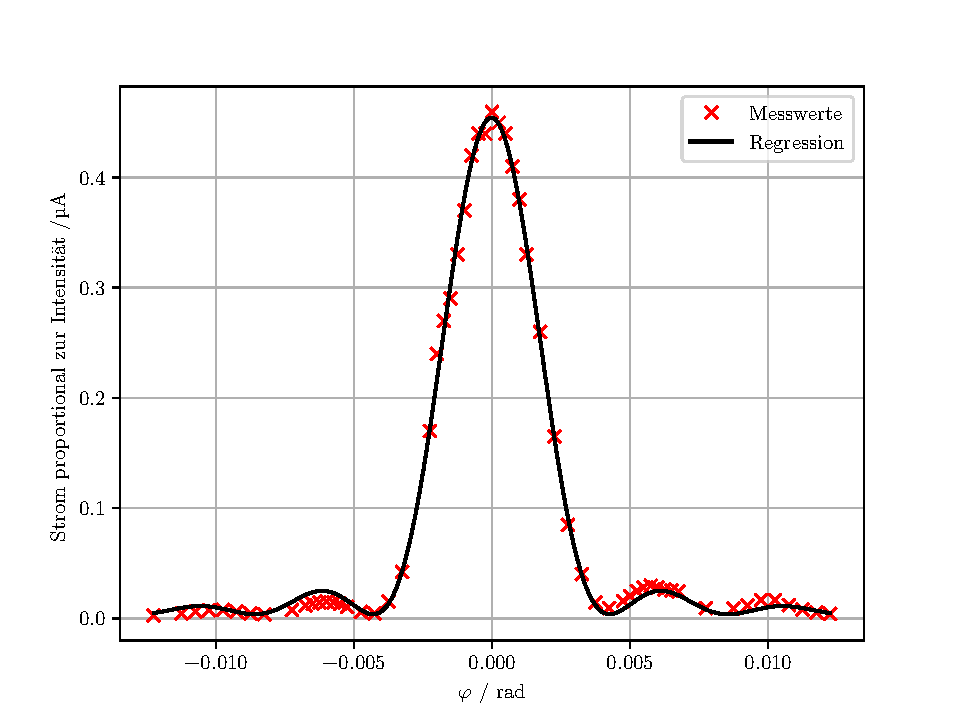
\includegraphics{plot1.pdf}
%  \caption{Darstellung der Messwerte sowie Regression.}
%  \label{abb:}
%\end{figure}
Die Regression wurde mit Python 3.6 durchgeführt.
Es folgt eine Winkelverschiebung von:
%\begin{equation*}
%  \Delta\phi =
%\end{equation*}
Somit ergibt sich mithilfe der Gleichung \ref{eq:} eine Spaltbreite von:
%\begin{equation*}
%  b_{mess} =
%\end{equation*}
Dies ist eine Abwichung von $0,00\%$ vom Literaturwert.
\subsection{Messung am einfach Spalt 2}
Das Verfahren ist die selbe wie beim Einfach Spalt 1. Es werden nun die Daten
in der Tabelle \ref{tab:2} dargestellt.
%\begin{table}[H]
%  \centering
%  \caption{Messdaten am einfach Spalt 1.}
%  \label{tab:2}
%  \begin{tabular}{c c c c}
%    \toprule
%    $x / \si{\milli\meter}$ & $I /\si{\mikro\ampre}$ &$x / \si{\milli\meter}$ & $I /\si{\mikro\ampre}$\\
%    \midrule
%    \bottomrule
%  \end{tabular}
%\end{table}
Mit den Daten aus Tabelle \ref{tab:2} werden sie gegeneinander aufgetragen und sind in der Abbildung
\ref{abb:} dargestellt.
%\begin{figure}[H]
%  \centering
%  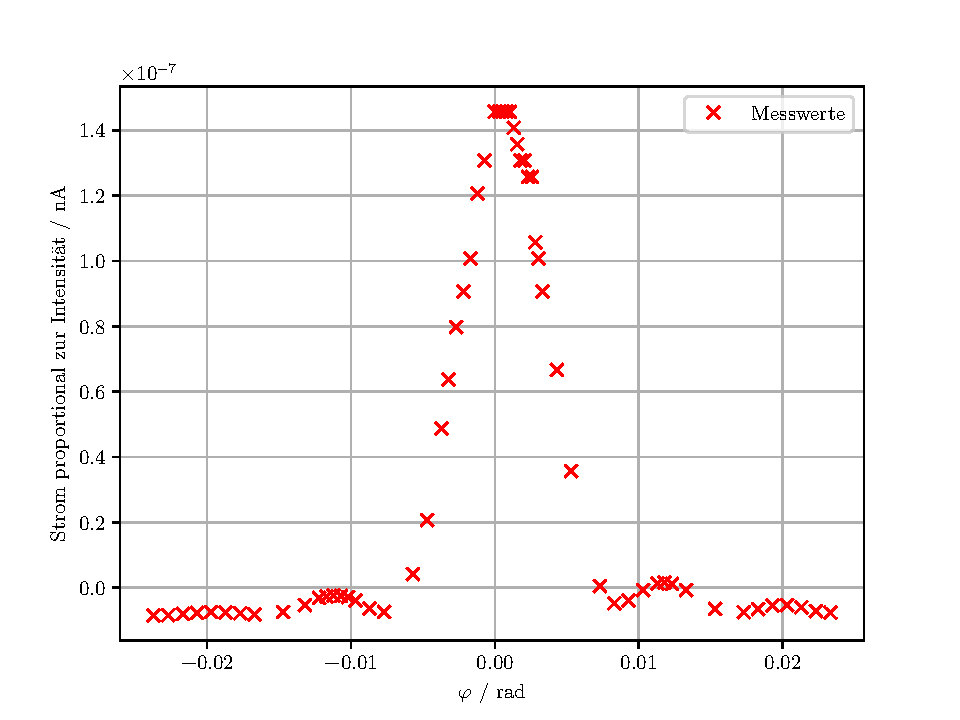
\includegraphics{plot2.pdf}
%  \caption{Darstellung der Messwerte sowie Regression.}
%  \label{abb:}
%\end{figure}
Die Regression wurde mit Python 3.6 durchgeführt.
Es folgt auch hier eine Winkelverschiebung von:
%\begin{equation*}
%  \Delta\phi =
%\end{equation*}
Somit ergibt sich mithilfe der Gleichung \ref{eq:} eine Spaltbreite von:
%\begin{equation*}
%  b_{mess} =
%\end{equation*}
Dies ist eine Abwichung von $0,00\%$ vom Literaturwert.
\subsection{Doppelspalt}
Auch hier werden die Daten aus der Tabelle \ref{tab:3} gegeneinander aufgetragen und in Abbildung
\ref{abb:} dargestellt.
%\begin{table}[H]
%  \centering
%  \caption{Messdaten am einfach Spalt 1.}
%  \label{tab:1}
%  \begin{tabular}{c c c c}
%    \toprule
%    $x / \si{\milli\meter}$ & $I /\si{\mikro\ampre}$ &$x / \si{\milli\meter}$ & $I /\si{\mikro\ampre}$\\
%    \midrule
%    \bottomrule
%  \end{tabular}
%\end{table}
%\begin{figure}[H]
%  \centering
%  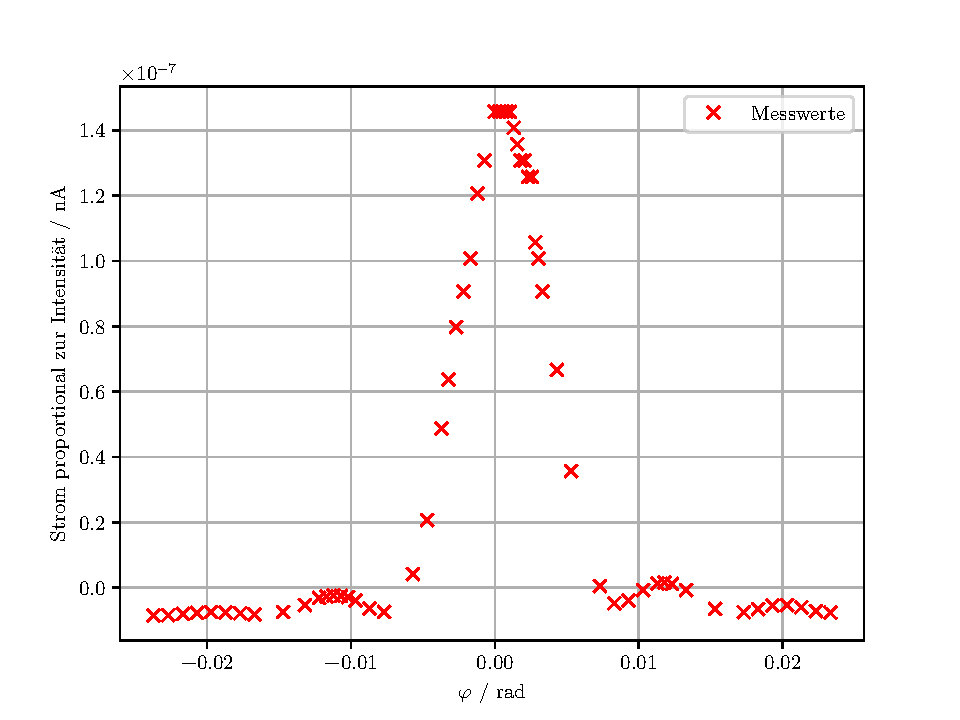
\includegraphics{plot2.pdf}
%  \caption{Darstellung der Messwerte sowie Regression.}
%  \label{abb:}
%\end{figure}
Die Regression wurde mit Python 3.6 durchgeführt.
Es folgt auch hier eine Winkelverschiebung von:
%\begin{equation*}
%  \Delta\phi =
%\end{equation*}
Somit ergibt sich mithilfe der Gleichung \ref{eq:} eine Spaltbreite von:
%\begin{equation*}
%  b_{mess} =
%\end{equation*}
Dies ist eine Abwichung von $0,00\%$ vom Literaturwert.
\subsection{Vergleich vom einfach Spalt mit Doppelspalt}
Die Daten aus Tabelle \ref{tab:} und \ref{tab:} werden nun in Abbildung \ref{abb:}
aufgetragen und verglichen.
%\begin{figure}[H]
%  \centering
%  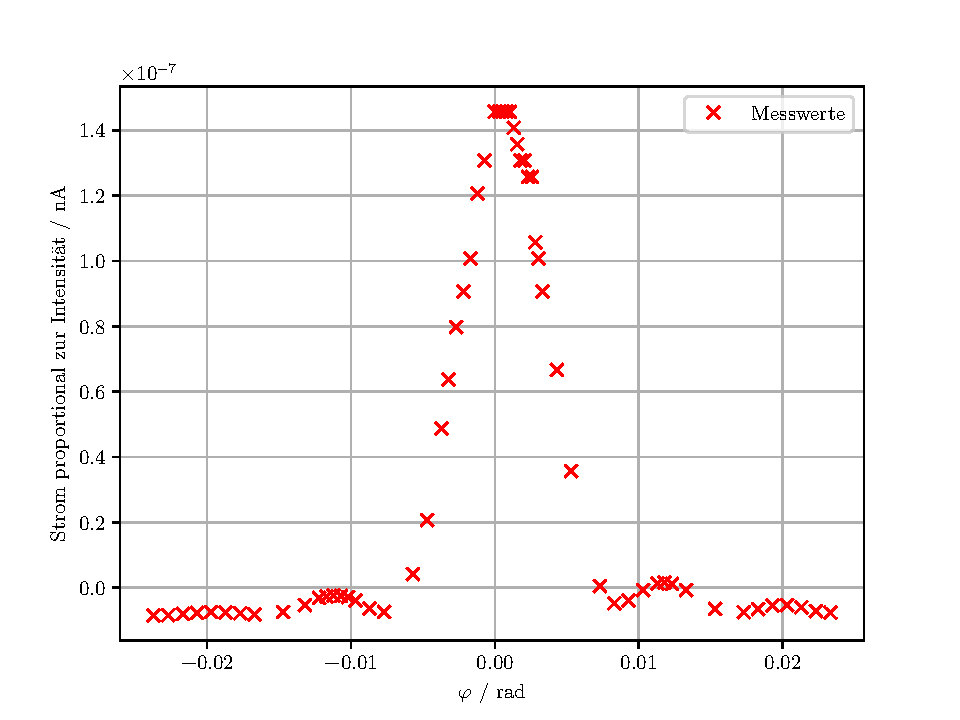
\includegraphics{plot2.pdf}
%  \caption{Darstellung der Messwerte sowie Regression.}
%  \label{abb:}
%\end{figure}
